\tikzset{every picture/.style={line width=0.75pt}} %set default line width to 0.75pt        

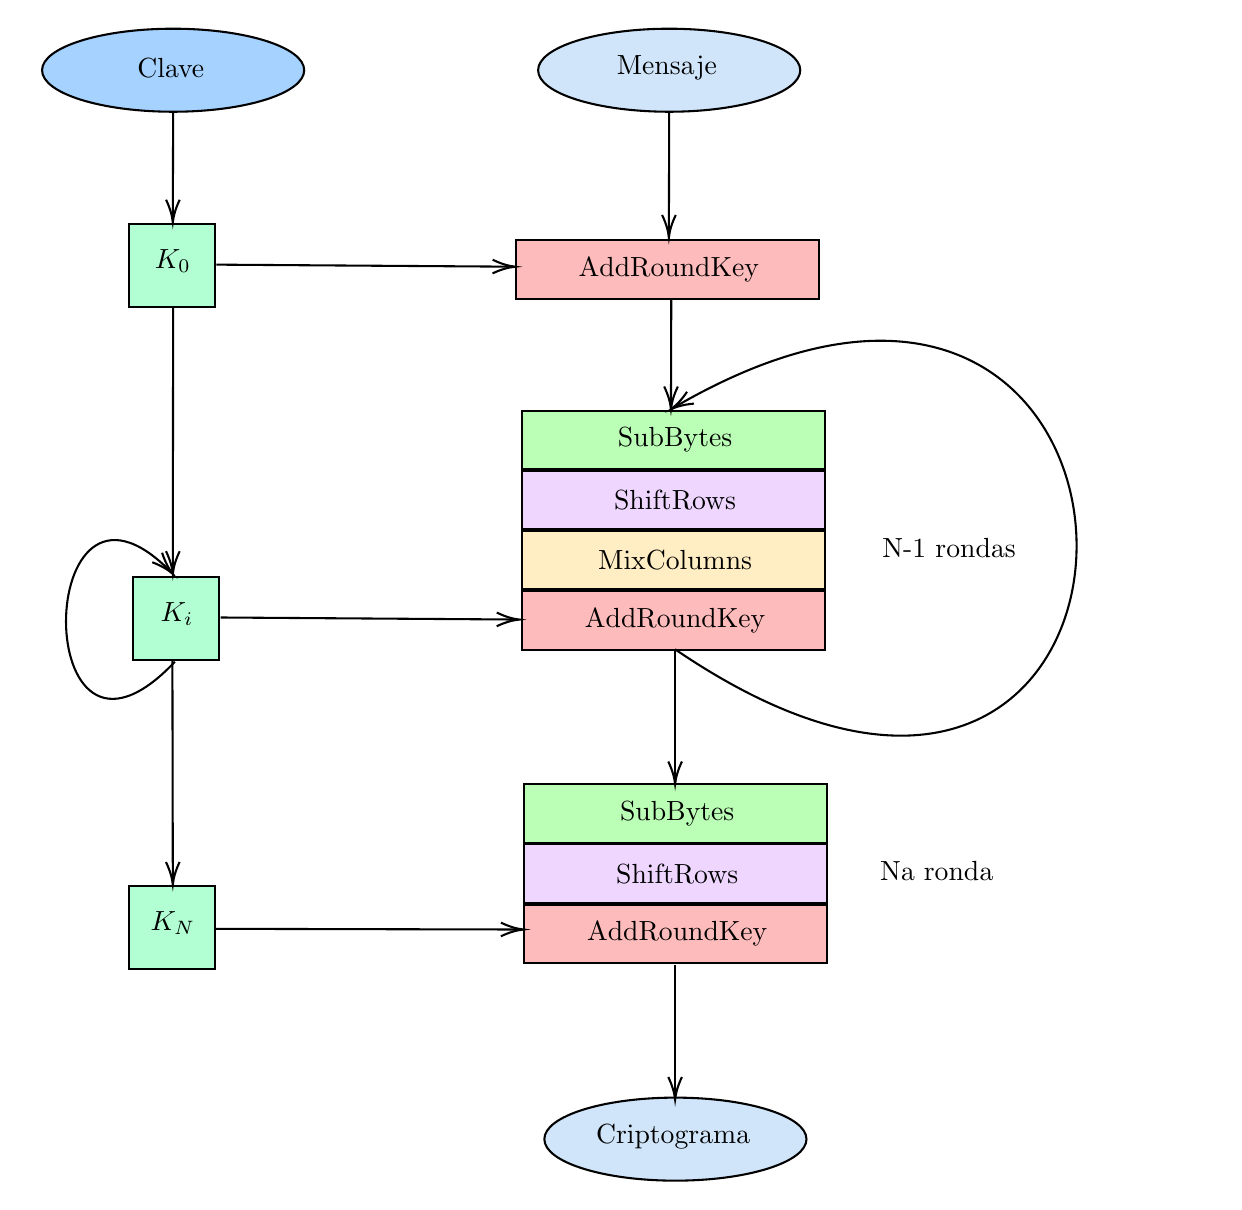
\begin{tikzpicture}[x=0.75pt,y=0.75pt,yscale=-1,xscale=1]
%uncomment if require: \path (0,607.4630661010742); %set diagram left start at 0, and has height of 607.4630661010742

%Shape: Ellipse [id:dp9737685907668199] 
\draw  [color={rgb, 255:red, 0; green, 0; blue, 0 }  ,draw opacity=1 ][fill={rgb, 255:red, 165; green, 210; blue, 255 }  ,fill opacity=1 ] (104,40) .. controls (104,28.95) and (132.27,20) .. (167.15,20) .. controls (202.03,20) and (230.3,28.95) .. (230.3,40) .. controls (230.3,51.05) and (202.03,60) .. (167.15,60) .. controls (132.27,60) and (104,51.05) .. (104,40) -- cycle ;

%Shape: Ellipse [id:dp45013119054902284] 
\draw  [color={rgb, 255:red, 0; green, 0; blue, 0 }  ,draw opacity=1 ][fill={rgb, 255:red, 208; green, 229; blue, 249 }  ,fill opacity=1 ] (343,40) .. controls (343,28.95) and (371.27,20) .. (406.15,20) .. controls (441.03,20) and (469.3,28.95) .. (469.3,40) .. controls (469.3,51.05) and (441.03,60) .. (406.15,60) .. controls (371.27,60) and (343,51.05) .. (343,40) -- cycle ;

%Shape: Rectangle [id:dp657856114899342] 
\draw  [fill={rgb, 255:red, 178; green, 255; blue, 211 }  ,fill opacity=1 ] (146,114) -- (187.3,114) -- (187.3,154) -- (146,154) -- cycle ;

%Shape: Rectangle [id:dp261406348143415] 
\draw  [fill={rgb, 255:red, 178; green, 255; blue, 211 }  ,fill opacity=1 ] (148,284) -- (189.3,284) -- (189.3,324) -- (148,324) -- cycle ;

%Shape: Rectangle [id:dp9188720632833878] 
\draw  [fill={rgb, 255:red, 178; green, 255; blue, 211 }  ,fill opacity=1 ] (146,433) -- (187.3,433) -- (187.3,473) -- (146,473) -- cycle ;

%Shape: Rectangle [id:dp25111749195065625] 
\draw  [fill={rgb, 255:red, 254; green, 187; blue, 187 }  ,fill opacity=1 ] (332.3,122) -- (478.3,122) -- (478.3,150.2) -- (332.3,150.2) -- cycle ;

%Shape: Rectangle [id:dp9024991354173098] 
\draw  [fill={rgb, 255:red, 187; green, 255; blue, 182 }  ,fill opacity=1 ] (335.3,204) -- (481.3,204) -- (481.3,232.2) -- (335.3,232.2) -- cycle ;

%Shape: Rectangle [id:dp6677044127286271] 
\draw  [fill={rgb, 255:red, 238; green, 214; blue, 255 }  ,fill opacity=1 ] (335.3,233) -- (481.3,233) -- (481.3,261.2) -- (335.3,261.2) -- cycle ;

%Shape: Rectangle [id:dp5668522361712407] 
\draw  [fill={rgb, 255:red, 255; green, 237; blue, 195 }  ,fill opacity=1 ] (335.3,262) -- (481.3,262) -- (481.3,290.2) -- (335.3,290.2) -- cycle ;

%Shape: Rectangle [id:dp34737624535273803] 
\draw  [fill={rgb, 255:red, 254; green, 187; blue, 187 }  ,fill opacity=1 ] (335.3,291) -- (481.3,291) -- (481.3,319.2) -- (335.3,319.2) -- cycle ;

%Shape: Rectangle [id:dp4367963290792771] 
\draw  [fill={rgb, 255:red, 187; green, 255; blue, 182 }  ,fill opacity=1 ] (336.3,384) -- (482.3,384) -- (482.3,412.2) -- (336.3,412.2) -- cycle ;

%Shape: Rectangle [id:dp012716397520244005] 
\draw  [fill={rgb, 255:red, 238; green, 214; blue, 255 }  ,fill opacity=1 ] (336.3,413) -- (482.3,413) -- (482.3,441.2) -- (336.3,441.2) -- cycle ;

%Shape: Rectangle [id:dp1945157717160817] 
\draw  [fill={rgb, 255:red, 254; green, 187; blue, 187 }  ,fill opacity=1 ] (336.3,442) -- (482.3,442) -- (482.3,470.2) -- (336.3,470.2) -- cycle ;

%Shape: Ellipse [id:dp0074509944076393] 
\draw  [color={rgb, 255:red, 0; green, 0; blue, 0 }  ,draw opacity=1 ][fill={rgb, 255:red, 208; green, 229; blue, 249 }  ,fill opacity=1 ] (346,555) .. controls (346,543.95) and (374.27,535) .. (409.15,535) .. controls (444.03,535) and (472.3,543.95) .. (472.3,555) .. controls (472.3,566.05) and (444.03,575) .. (409.15,575) .. controls (374.27,575) and (346,566.05) .. (346,555) -- cycle ;

%Straight Lines [id:da2019009163904124] 
\draw    (167.15,60) -- (167.01,111.33) ;
\draw [shift={(167,113.33)}, rotate = 270.15999999999997] [color={rgb, 255:red, 0; green, 0; blue, 0 }  ][line width=0.75]    (10.93,-3.29) .. controls (6.95,-1.4) and (3.31,-0.3) .. (0,0) .. controls (3.31,0.3) and (6.95,1.4) .. (10.93,3.29)   ;

%Straight Lines [id:da7298574790525367] 
\draw    (406.15,60) -- (406,118.67) ;
\draw [shift={(406,120.67)}, rotate = 270.14] [color={rgb, 255:red, 0; green, 0; blue, 0 }  ][line width=0.75]    (10.93,-3.29) .. controls (6.95,-1.4) and (3.31,-0.3) .. (0,0) .. controls (3.31,0.3) and (6.95,1.4) .. (10.93,3.29)   ;

%Straight Lines [id:da12255807726786161] 
\draw    (188,133.67) -- (330,134.65) ;
\draw [shift={(332,134.67)}, rotate = 180.4] [color={rgb, 255:red, 0; green, 0; blue, 0 }  ][line width=0.75]    (10.93,-3.29) .. controls (6.95,-1.4) and (3.31,-0.3) .. (0,0) .. controls (3.31,0.3) and (6.95,1.4) .. (10.93,3.29)   ;

%Straight Lines [id:da15131688097810092] 
\draw    (407.15,150) -- (407.01,201.33) ;
\draw [shift={(407,203.33)}, rotate = 270.15999999999997] [color={rgb, 255:red, 0; green, 0; blue, 0 }  ][line width=0.75]    (10.93,-3.29) .. controls (6.95,-1.4) and (3.31,-0.3) .. (0,0) .. controls (3.31,0.3) and (6.95,1.4) .. (10.93,3.29)   ;

%Straight Lines [id:da5876036775611393] 
\draw    (190,303.67) -- (332,304.65) ;
\draw [shift={(334,304.67)}, rotate = 180.4] [color={rgb, 255:red, 0; green, 0; blue, 0 }  ][line width=0.75]    (10.93,-3.29) .. controls (6.95,-1.4) and (3.31,-0.3) .. (0,0) .. controls (3.31,0.3) and (6.95,1.4) .. (10.93,3.29)   ;

%Straight Lines [id:da031674005498631086] 
\draw    (167.15,154) -- (167,280.67) ;
\draw [shift={(167,282.67)}, rotate = 270.07] [color={rgb, 255:red, 0; green, 0; blue, 0 }  ][line width=0.75]    (10.93,-3.29) .. controls (6.95,-1.4) and (3.31,-0.3) .. (0,0) .. controls (3.31,0.3) and (6.95,1.4) .. (10.93,3.29)   ;

%Curve Lines [id:da11017760368079688] 
\draw    (409,319) .. controls (666.24,494.29) and (668.24,49.29) .. (407,203.33) ;
\draw [shift={(407,203.33)}, rotate = 329.47] [color={rgb, 255:red, 0; green, 0; blue, 0 }  ][line width=0.75]    (10.93,-3.29) .. controls (6.95,-1.4) and (3.31,-0.3) .. (0,0) .. controls (3.31,0.3) and (6.95,1.4) .. (10.93,3.29)   ;

%Curve Lines [id:da7191324048148082] 
\draw    (168,325) .. controls (97.57,399.34) and (99.2,213.59) .. (165.99,281.62) ;
\draw [shift={(167,282.67)}, rotate = 226.31] [color={rgb, 255:red, 0; green, 0; blue, 0 }  ][line width=0.75]    (10.93,-3.29) .. controls (6.95,-1.4) and (3.31,-0.3) .. (0,0) .. controls (3.31,0.3) and (6.95,1.4) .. (10.93,3.29)   ;

%Straight Lines [id:da034441479180648216] 
\draw    (166.8,324.33) -- (167,430.4) ;
\draw [shift={(167,432.4)}, rotate = 269.89] [color={rgb, 255:red, 0; green, 0; blue, 0 }  ][line width=0.75]    (10.93,-3.29) .. controls (6.95,-1.4) and (3.31,-0.3) .. (0,0) .. controls (3.31,0.3) and (6.95,1.4) .. (10.93,3.29)   ;

%Straight Lines [id:da40164122139794234] 
\draw    (409,319) -- (409,382) ;
\draw [shift={(409,384)}, rotate = 270] [color={rgb, 255:red, 0; green, 0; blue, 0 }  ][line width=0.75]    (10.93,-3.29) .. controls (6.95,-1.4) and (3.31,-0.3) .. (0,0) .. controls (3.31,0.3) and (6.95,1.4) .. (10.93,3.29)   ;

%Straight Lines [id:da19063932307712084] 
\draw    (187,453.67) -- (334,454) ;
\draw [shift={(336,454)}, rotate = 180.13] [color={rgb, 255:red, 0; green, 0; blue, 0 }  ][line width=0.75]    (10.93,-3.29) .. controls (6.95,-1.4) and (3.31,-0.3) .. (0,0) .. controls (3.31,0.3) and (6.95,1.4) .. (10.93,3.29)   ;

%Straight Lines [id:da027755398290204125] 
\draw    (409,471) -- (409,534) ;
\draw [shift={(409,536)}, rotate = 270] [color={rgb, 255:red, 0; green, 0; blue, 0 }  ][line width=0.75]    (10.93,-3.29) .. controls (6.95,-1.4) and (3.31,-0.3) .. (0,0) .. controls (3.31,0.3) and (6.95,1.4) .. (10.93,3.29)   ;


% Text Node
\draw (166,39) node  [align=left] {Clave};
% Text Node
\draw (405,39) node  [align=left] {Mensaje};
% Text Node
\draw (167,132) node   {$K_{0}$};
% Text Node
\draw (169,302) node   {$K_{i}$};
% Text Node
\draw (167,451) node   {$K_{N}$};
% Text Node
\draw (406,136) node  [align=left] {AddRoundKey};
% Text Node
\draw (409,218) node  [align=left] {SubBytes};
% Text Node
\draw (409,247) node  [align=left] {ShiftRows};
% Text Node
\draw (409,276) node  [align=left] {MixColumns};
% Text Node
\draw (409,305) node  [align=left] {AddRoundKey};
% Text Node
\draw (410,456) node  [align=left] {AddRoundKey};
% Text Node
\draw (410,427) node  [align=left] {ShiftRows};
% Text Node
\draw (410,398) node  [align=left] {SubBytes};
% Text Node
\draw (408,554) node  [align=left] {Criptograma};
% Text Node
\draw (541,270) node  [align=left] {N-1 rondas};
% Text Node
\draw (535,426) node  [align=left] {Na ronda};


\end{tikzpicture}
